\section{Coletas de Dados com os Pacientes}

    As coletas de dados foram implementadas seguindo uma estrutura de ficha, definida a partir das normas de avaliação CIF. Sendo assim, todas as coletas de dados seguiram a seguinte ordem, também descrita na Figura 7:

    \begin{itemize}
        \item Acolhimento do paciente e coleta de seus dados pessoais;
        \item Aplicação da ficha de avaliação do paciente, feita por um profissional da área de saúde;
        \item Sessão de fotos do coto e do paciente para futura análise postural e de condição da pele.
    \end{itemize}

    \begin{figure}[ht]
        \centering
        \label{fig07}
            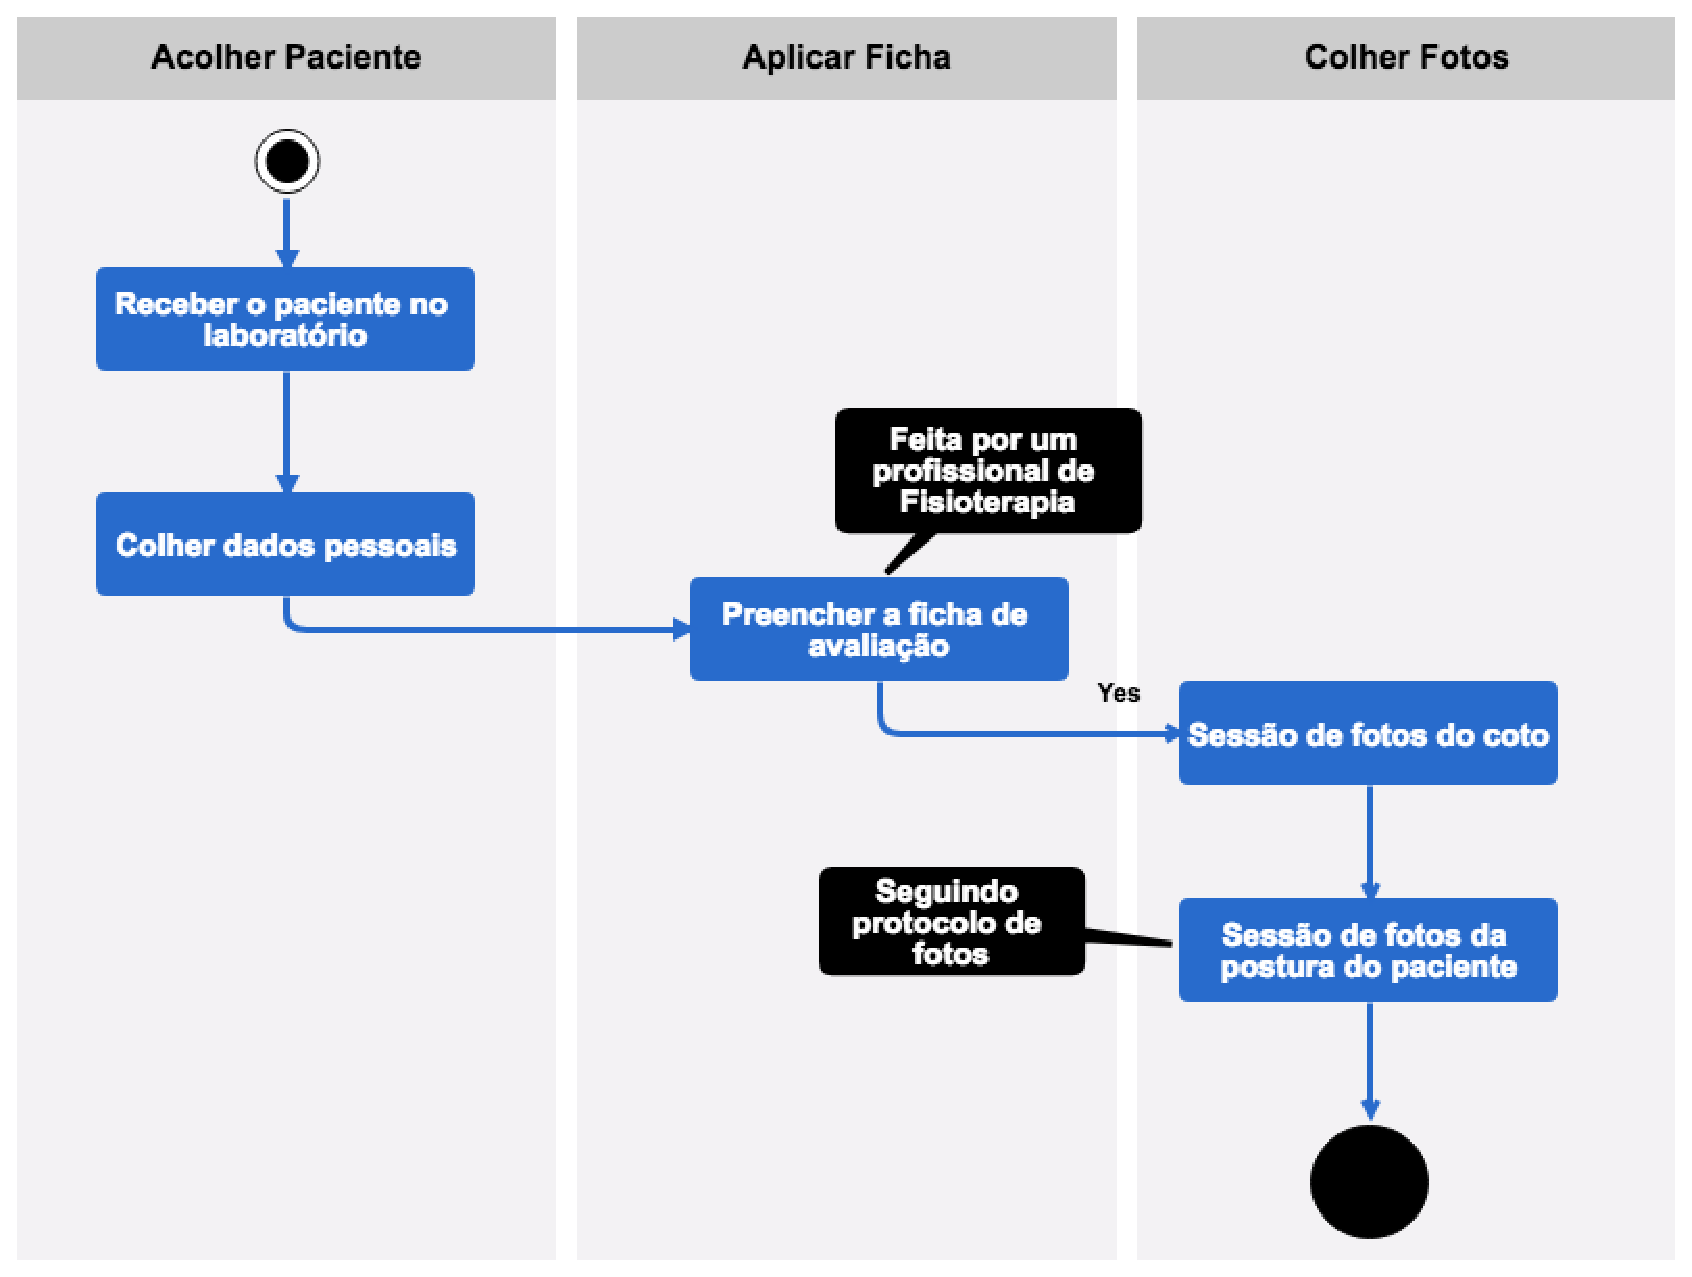
\includegraphics[keepaspectratio=true, scale=0.4]{editaveis/images/colet_flow.eps}
        \caption{Fluxo de trabalho da coleta}
    \end{figure}

    A sessão de fotos faz parte de um protocolo estabelecido, sendo padronizado em aspectos de posicionamento semelhantes ao de \cite{Barauna2006}, visto que todas as fotos dos cotos dos pacientes precisam estar sob a mesma condição de iluminação. Desta forma, a Figura 8 mostra o fluxo de trabalho para recolhimento das fotografias. O protocolo desenvolvido e utilizado em todas as sessões de fotos foi:

    \begin{itemize}
        \item Utilização da mesma câmera fotográfica em todas as fotografias tiradas;
        \item Utilização de um pano do tipo TNT branco para plano de fundo;
        \item Utilização de uma luz frontal branca posicionada na parte de baixo da câmera;
        \item A fotografia foi tirada enquadrando ao centro da grade da câmera a maior parte possível do coto, sem mostrar qualquer plano de fundo;
        \item As fotografias dos cotos foram tiradas em três ângulos diferentes, sendo eles um frontal, um lateral e, um último, frontal do coto com solicitação de flexão de quadril (a 90 graus em relação ao solo).
    \end{itemize}

    \begin{figure}[ht]
        \centering
        \label{fig08}
            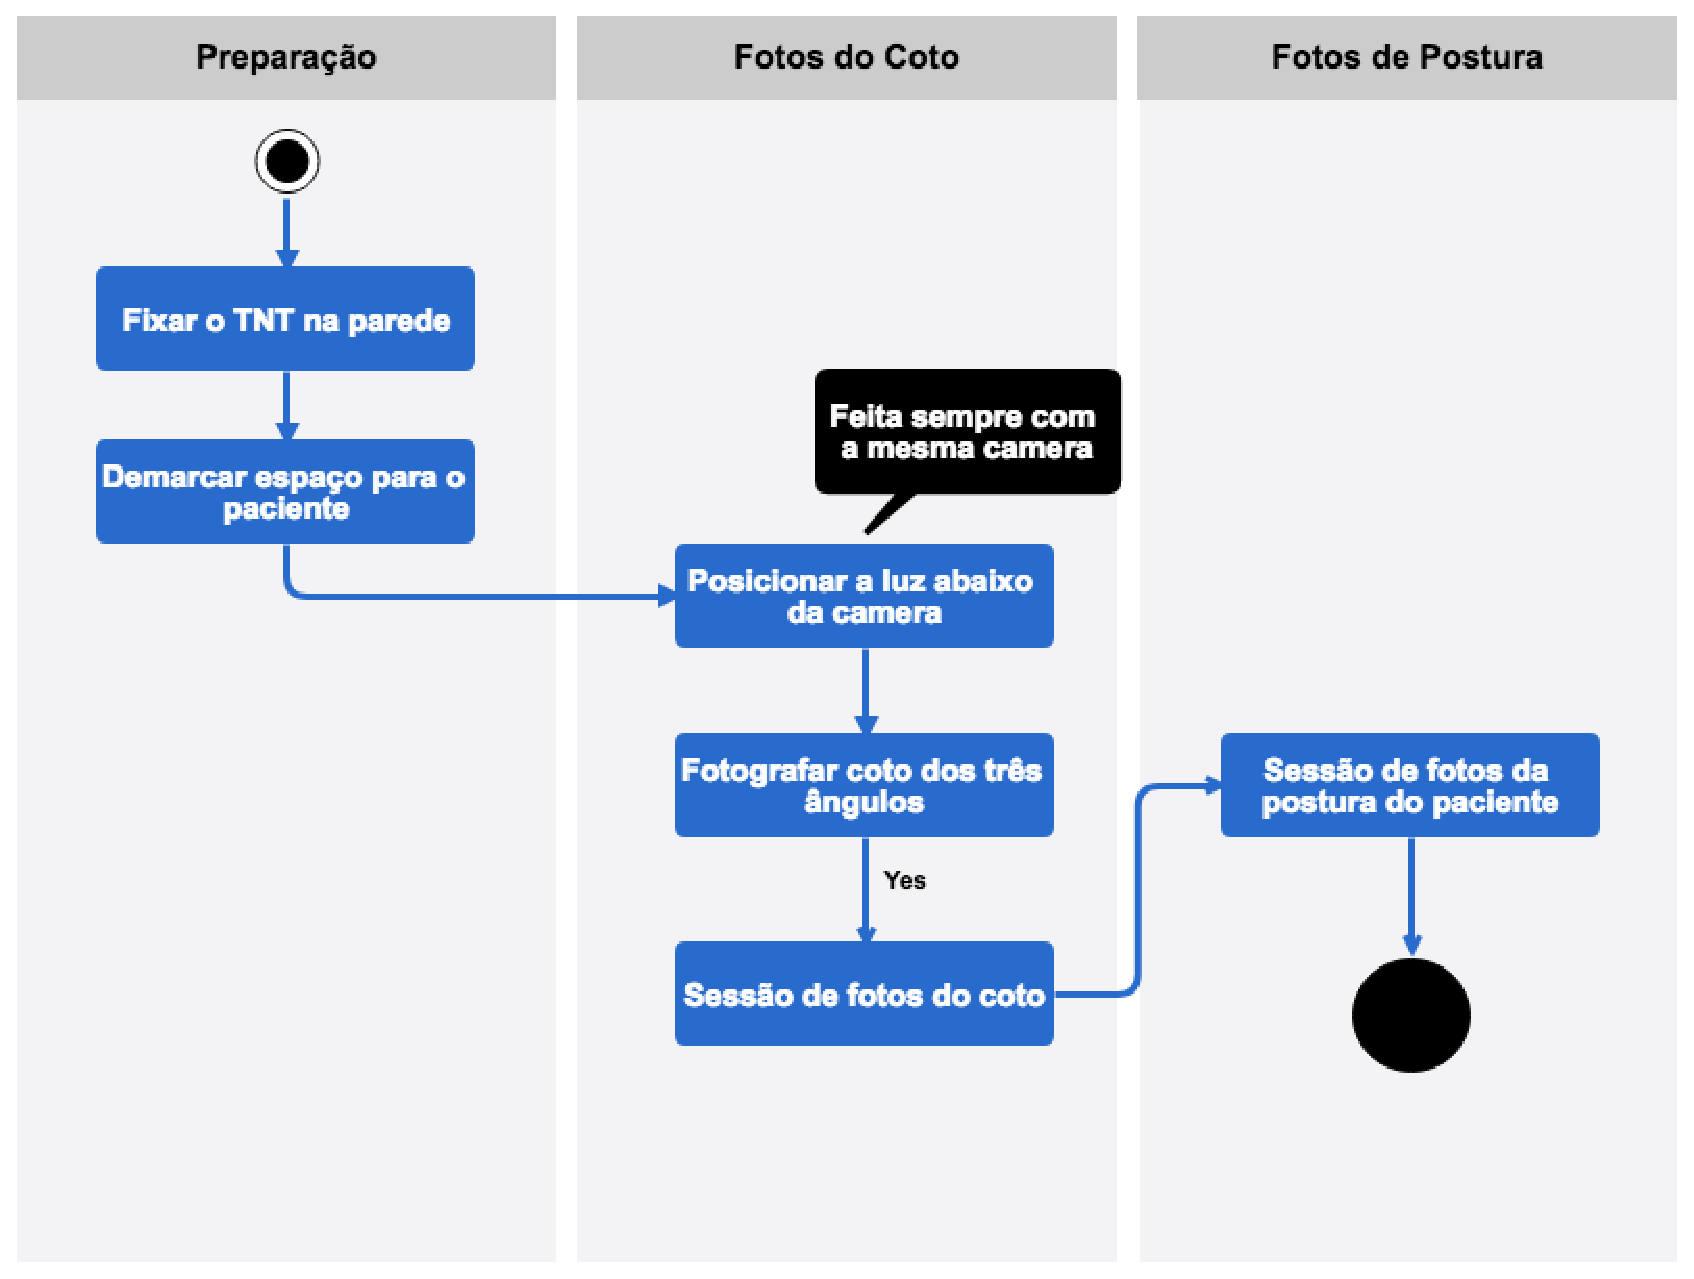
\includegraphics[keepaspectratio=true, scale=0.4]{editaveis/images/fotos_flow.eps}
        \caption{Fluxo de trabalho das fotografias}
    \end{figure}


\section{Modelo de Machine Learning}

    Tendo como meta a definição de um modelo de ML para ser aplicada em uma RNA a ser treinada para detecção de tipos de pele, a estratégia a ser seguida foi o fluxo de trabalho de aprendizado de máquinas, descrito na Figura 6 e adaptado para esta aplicação como mostra a Figura 9.

    \begin{figure}[ht]
        \centering
        \label{fig09}
            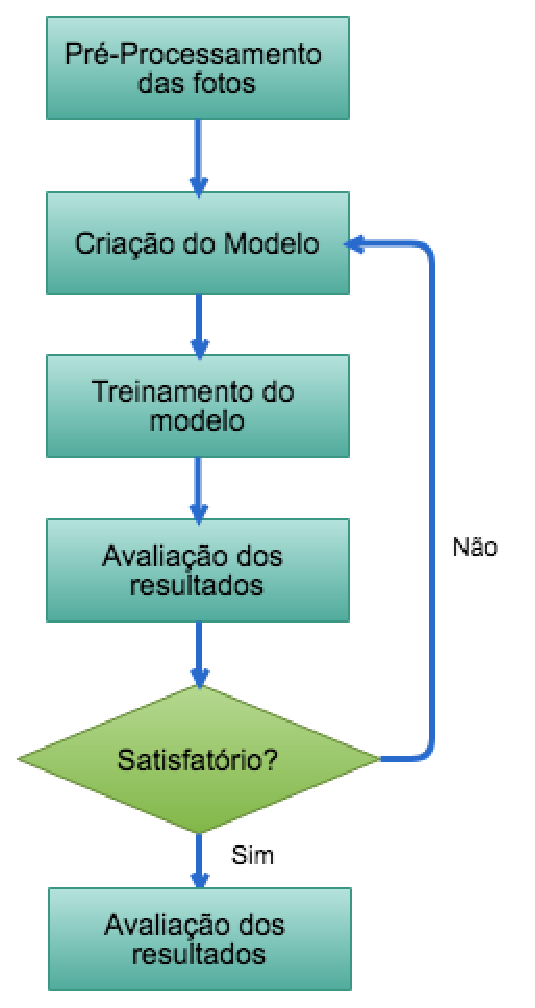
\includegraphics[keepaspectratio=true, scale=0.4]{editaveis/images/ml_nt_flow.eps}
        \caption{Fluxo de trabalho da construção do modelo de ML}
    \end{figure}

    \subsection{Construção do Modelo}

        O modelo de aprendizado utilizado é o supervisionado, baseado em uma RNA MLP com método de treinamento \textit{backpropagation}.
        Sendo assim, os passos a serem seguidos para a construção do modelo inicial são:

        \begin{itemize}
            \item Pré-processamento dos dados: \\ Neste primeiro passo, é montado o modelo de dados de treinamento que será usado para apresentação e utilização dos dados. Para isso é necessário encontrar uma correlação entre os dados de entrada e o dado a ser atingido pelo processo de aprendizado.

            \item Criação do modelo: \\ O modelo deve ser criado para receber os dados de entrada como pré-processados fazer seu processamento visando o resultado a ser obtido.

            \item Treinamento do modelo: \\ O modelo proposto deve passar por um breve treinamento para que os erros sejam corrigidos antes que a rede comece a rebeber dados para serem analisados.

            \item Avaliar o modelo: \\ Uma vez com o modelo pronto é necessário avaliar a aplicabilidade do modelo em vista da acurácia obtida em relação a quantidade de reconhecimentos feitos em uma base de dados controlada e com um número conhecido de dados coletados dos pacientes.

            \item Apresentar resultados: \\ Assim que o modelo é avaliado, se for julgado com resultado insatisfatório ele deve ser reencaminhado para uma melhoria na modelagem, caso seja satisfatório, devem ser apresentados aqui os resultados obtidos.
        \end{itemize}
